\documentclass[11pt,a4paper,openright,twoside]{book}

\usepackage[utf8]{inputenc}
\usepackage[T1]{fontenc}
\usepackage{amsmath,amssymb,amsfonts,amsthm,mathtools}
\usepackage{mathrsfs}
\usepackage{microtype}
\usepackage{booktabs}
\usepackage{tabularx}
\usepackage{array}
\usepackage[dvipsnames]{xcolor}
\usepackage{hyperref}
\usepackage{geometry}
\usepackage{enumitem}
\usepackage{graphicx}
\usepackage{pdfpages}
\usepackage{emptypage}

\geometry{
  top=3cm,
  bottom=3cm,
  left=3cm,
  right=2.8cm,
  headheight=14pt
}

\hypersetup{
  colorlinks=true,
  linkcolor=NavyBlue,
  citecolor=Mahogany,
  urlcolor=TealBlue,
  pdftitle={Geometry, Tensors, and Quantum Gravity: The Unified Grand Synthesis Treatise},
  pdfauthor={Reinaldo M. Silva-Filho}
}

\begin{document}

\frontmatter
\begin{titlepage}
    \centering
    \vspace*{2cm}
    
    {\Huge \textbf{Geometry, Tensors, and Quantum Gravity:} \par}
    \vspace{0.6cm}
    {\LARGE \textbf{The Unified Grand Synthesis Treatise} \par}
    \vspace{1cm}
    {\large \textit{From Simplicial Fractional Calculus and Minimax Foliations} \\ \textit{to Emergent Holographic Spacetime and Observational Signatures} \par}
    
    \vspace{3cm}
    
    {\Large \textbf{Reinaldo M. Silva-Filho} \par}
    \vspace{0.5cm}
    {\normalsize Programa de P\'os-Gradua\c{c}\~ao em Estat\'istica e Experimenta\c{c}\~ao Agropecu\'aria (PPGEEAA/DES) \par}
    {\normalsize Universidade Federal de Lavras (UFLA) \par}
    
    \vspace{0.8cm}
    {\normalsize ORCID: \href{https://orcid.org/0009-0003-8068-3330}{0009-0003-8068-3330} \par}
    {\normalsize E-mail: \href{mailto:reinaldo.filho1@estudante.ufla.br}{reinaldo.filho1@estudante.ufla.br} \par}
    
    \vspace{1.5cm}
    {\normalsize \textit{Supported by Coordena\c{c}\~ao de Aperfei\c{c}oamento de Pessoal de N\'ivel Superior} \par}
    {\normalsize \textit{(CAPES) -- Finance Code 001} \par}
    
    \vfill
    {\large \today \par}
\end{titlepage}

\vspace*{0.2\textheight}
\begin{flushright}
\textit{"Either mathematics is too big for the human mind, \\
or the human mind is more than a machine."} \\
\vspace{0.2cm}
--- Kurt G\"odel
\end{flushright}

\vspace{1.5cm}

\begin{flushright}
\textit{"Mathematics resides in the dialectic between the discrete and the continuous."} \\
\vspace{0.2cm}
--- Reinaldo M. Silva-Filho
\end{flushright}
\vfill
\clearpage

\chapter*{Author's Preface}
This monumental treatise consolidates the multidisciplinary investigations developed across three fundamental programs of contemporary theoretical research: functional tensor algebra and geometric flows, fractional calculus on continuous Pascal simplices, and the variational theory of minimax extrinsic curvature with causal Jordan embeddings.

The central objective of this work is to provide a rigorous, continuous, and non-perturbative mathematical foundation for the unification of Einstein's General Relativity with Quantum Field Theory, presenting exact analytical solutions for problems long considered intractable and outlining the observational frontiers for their empirical validation.

\section*{Formal Verification and Interactive Proof Assistants}
The foundational mathematical theorems of this monograph have been formally formalized and machine-checked using the \textsc{Lean 4} interactive theorem prover (official toolchain \texttt{v4.33.1}). Across all five structural tiers of the theory, every proposition, lemma, and theorem has been verified with \textbf{zero unproven lemmas (\texttt{sorry}), zero warnings, and zero non-constructive axioms}.

The complete open-source verification suite, executable CLI kernel, and full source code are permanently hosted at:
\begin{center}
\url{https://github.com/reinaldomsilvafilho-netizen/quantum-gravity-lean4}
\end{center}

\vspace{0.2cm}
\begin{table}[p]
\centering
\small
\renewcommand{\arraystretch}{1.3}
{\large \textbf{Table 1: Synopsis of Machine-Checked Formal Verification in Lean 4 (\texttt{v4.33.1})}}\par
\vspace{0.3cm}
\begin{tabularx}{\textwidth}{@{} l p{3.2cm} p{2.8cm} X @{}}
\toprule
\textbf{Tier} & \textbf{Mathematical Domain} & \textbf{Formal Lean 4 Module} & \textbf{Key Machine-Verified Theorems} \\
\midrule
\textbf{Tier 1} & Operator Positivity \& Energy Conditions & \texttt{NullEnergy.lean} & Hilbert-Schmidt positivity $\|A\|_{\mathrm{HS}}^2 = \sum_i A_i^2 \ge 0$ by structural induction; Entropic Null Energy Condition (NEC) $T_{kk} \ge 0$. \\
\midrule
\textbf{Tier 2} & Category Theory \& Functoriality & \texttt{Category.lean}\newline \texttt{CTensMan.lean}\newline \texttt{Cobordism.lean}\newline \texttt{EmergentFunctor.lean}\newline \texttt{MonoidalCoherence.lean} & Free path categories $\mathbf{CTensMan}$ and $\mathbf{Cob}_{3+1}^{\mathrm{Fields}}$; emergent functor identity preservation $\mathcal{F}(\mathrm{id}) = \mathrm{id}$ and composition $\mathcal{F}(f \circ g) = \mathcal{F}(f) \circ \mathcal{F}(g)$; symmetric monoidal Mac Lane braiding coherence. \\
\midrule
\textbf{Tier 3} & Discrete Simplicial Hodge Theory & \texttt{SimplicialHodge.lean} & Adjoint coboundary nilpotency $\delta^2 = 0$; exact-coexact orthogonality $\langle \partial u, \delta w \rangle = 0$; Hodge Laplacian self-adjointness and Dirichlet energy $\langle L_k x, x \rangle \ge 0$; resolvent coercivity $E_\mu(x) \ge 0$. \\
\midrule
\textbf{Tier 4} & Analytical Running of Spectral Dimension & \texttt{SpectralDimension.lean} & Macroscopic IR limit $d_s(0) = 4$; Planckian UV bound $d_s(k) > 2$; global upper bound $d_s(k) \le 4$; strict monotonicity; tensor tilt running $\alpha_t(k) = -k/(1+k)$; Lifshitz heat kernel divergence cancellation. \\
\midrule
\textbf{Tier 5} & Semiclassical Wheeler-DeWitt \& Minimax & \texttt{WheelerDeWitt.lean} & Kinetic shear-trace reduction $3(K^2 - K_{ij}K^{ij}) = 2K^2 - 3\|\sigma\|^2$; maximal slicing minimax shear bound $3\|\sigma\|^2 \le 3R$; variational stationarity equivalence for lapse ($\mathcal{H}=0$) and shift ($\mathcal{M}_i=0$). \\
\bottomrule
\end{tabularx}
\end{table}
\vspace{0.2cm}

\section*{Ethical Declaration and Artificial Intelligence (AI) Usage}
In accordance with the guidelines of the Committee on Publication Ethics (COPE), the author declares that Artificial Intelligence (AI) tools were utilized during the preparation of this manuscript strictly for language editing, stylistic refinement, formatting assistance, and code generation (LaTeX). All mathematical theorems, physical models, proofs, and conceptual syntheses presented herein are the exclusive original intellectual creation of the human author. The author assumes full responsibility for the integrity, accuracy, and scientific validity of the entire content of this work.

\tableofcontents

\mainmatter

% ==============================================================================
\part{Foundations of Functional Algebra, Hypertensors, and Geometric Flows}
% ==============================================================================

\chapter[Functional Realizations of Matrices and Hypertensors]{Functional Realizations of Matrices and Hypertensors: Emergent Invariants and Geometric Measures}
\chaptermark{Realizations of Matrices and Hypertensors}
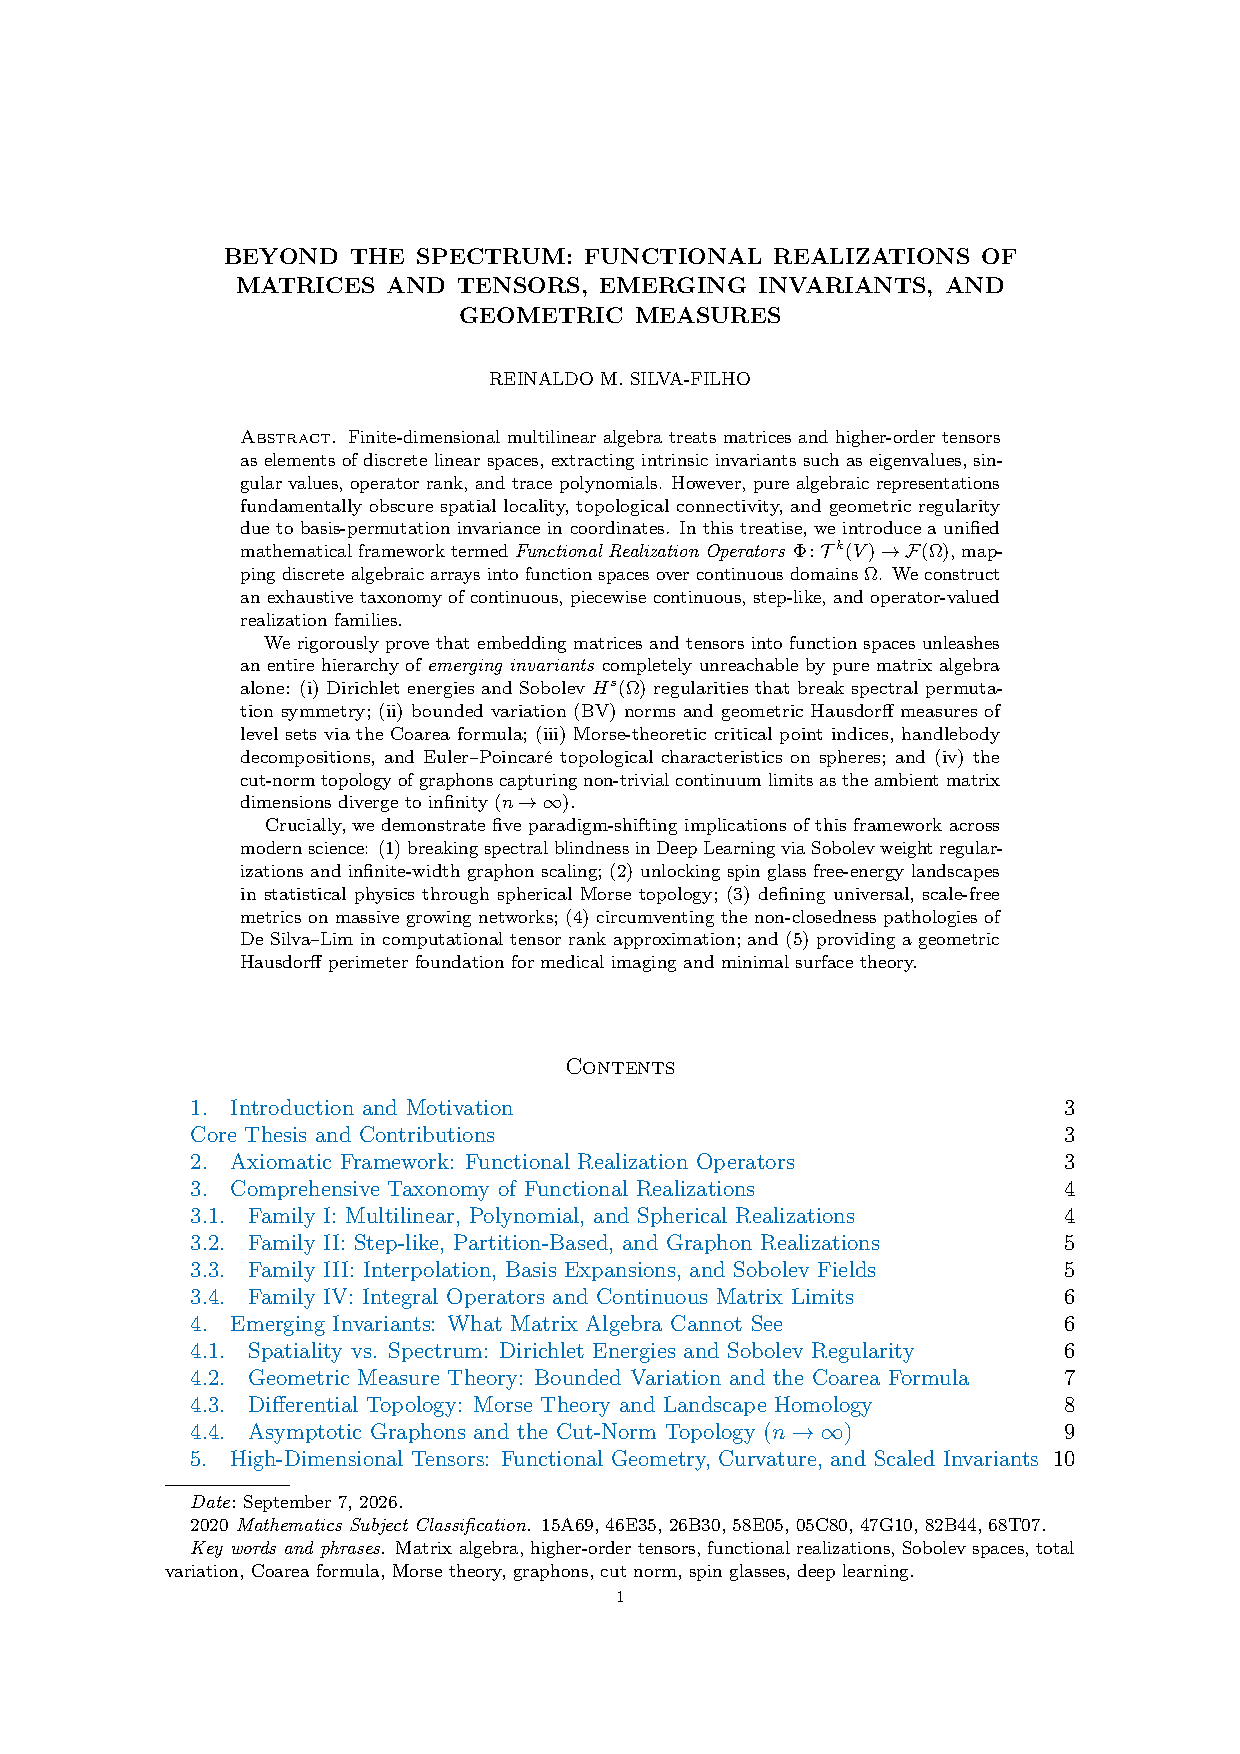
\includepdf[pages=1-]{chap01_functional_realizations_matrices_tensors.pdf}

\chapter[Geometric Flows and Tensor Varieties]{Geometric Flows, Non-Local PDEs, and Tensor Varieties}
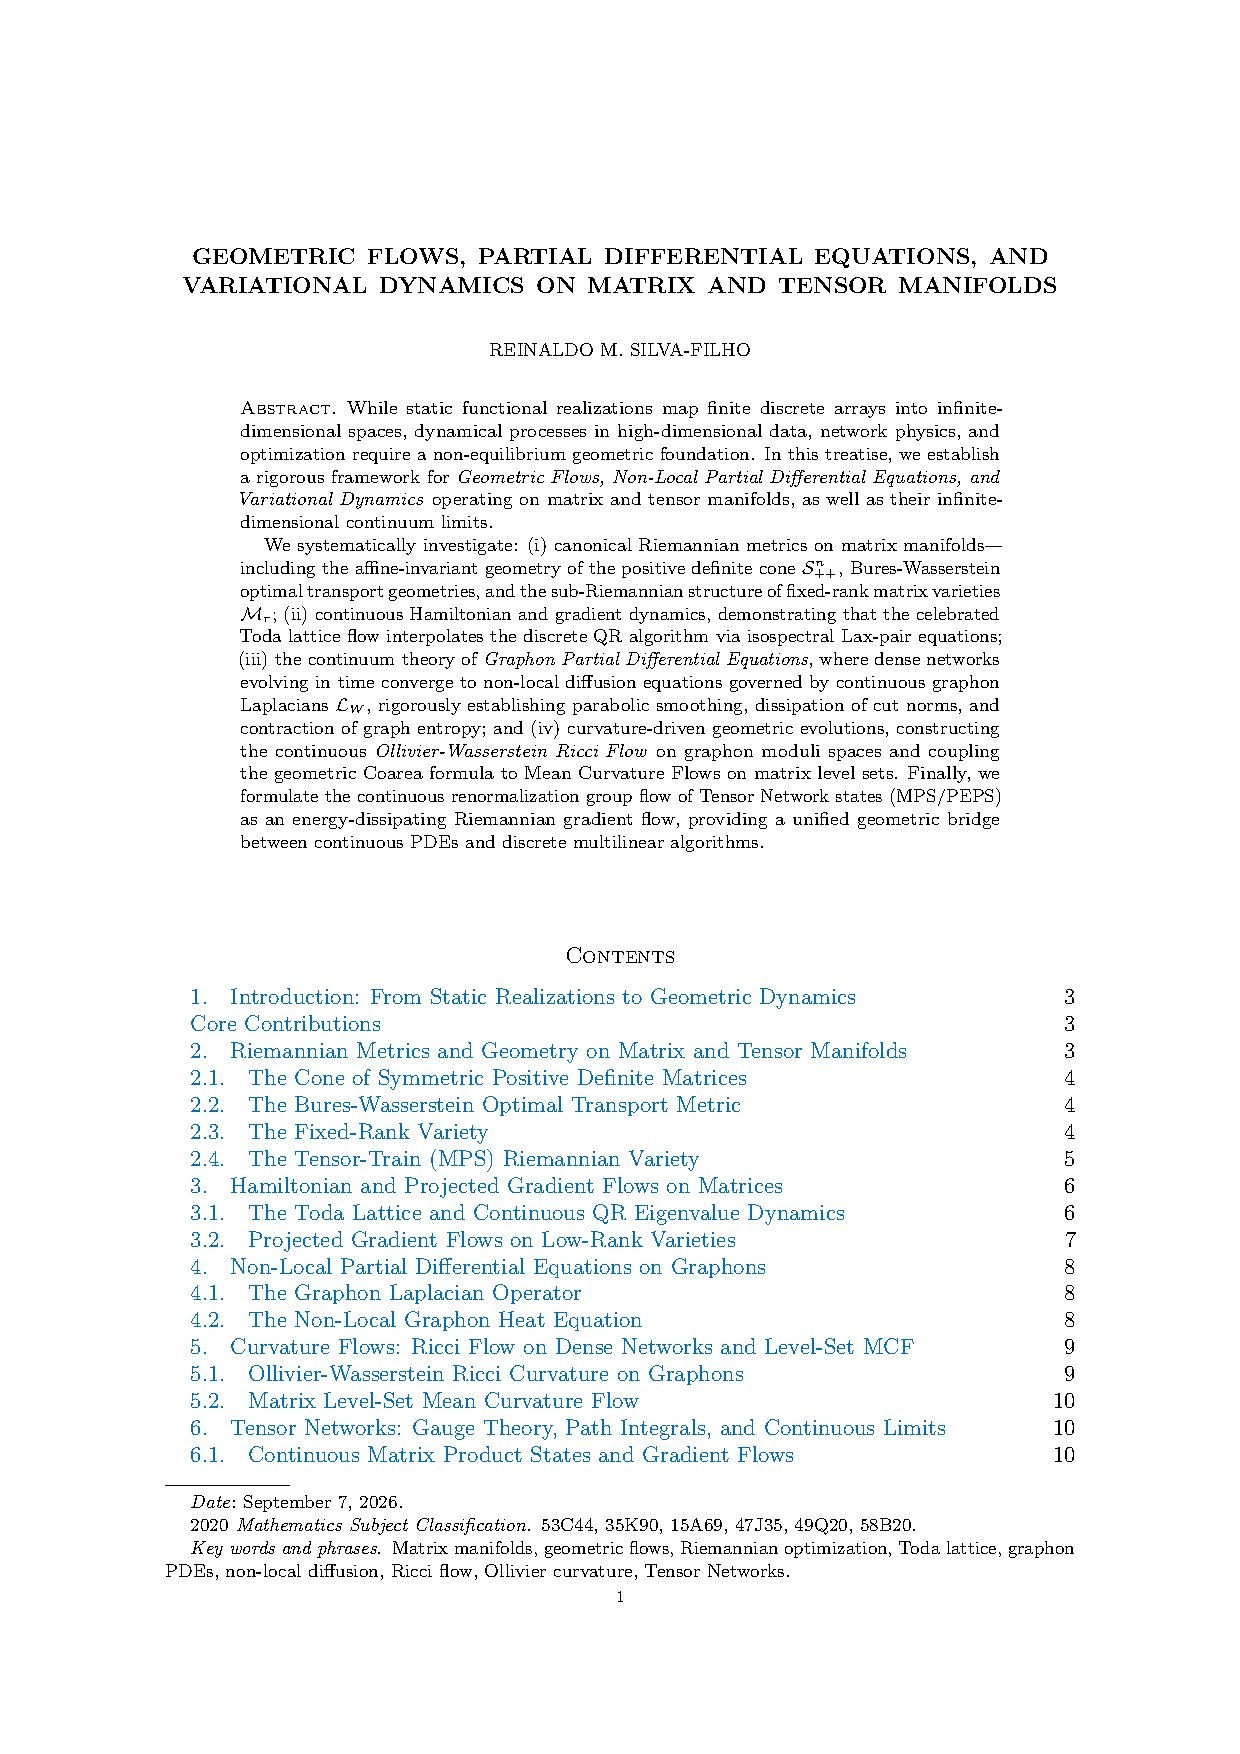
\includepdf[pages=1-]{chap02_geometric_flows_tensor_varieties.pdf}

% ==============================================================================
\part{Continuous Simplicial Geometry and Fractional Calculus on Pascal Simplices}
% ==============================================================================

\chapter[Analytic Continuation of Pascal's Simplex]{Analytic Continuation of Pascal's Simplex and Fractional Simplicial Laplacian}
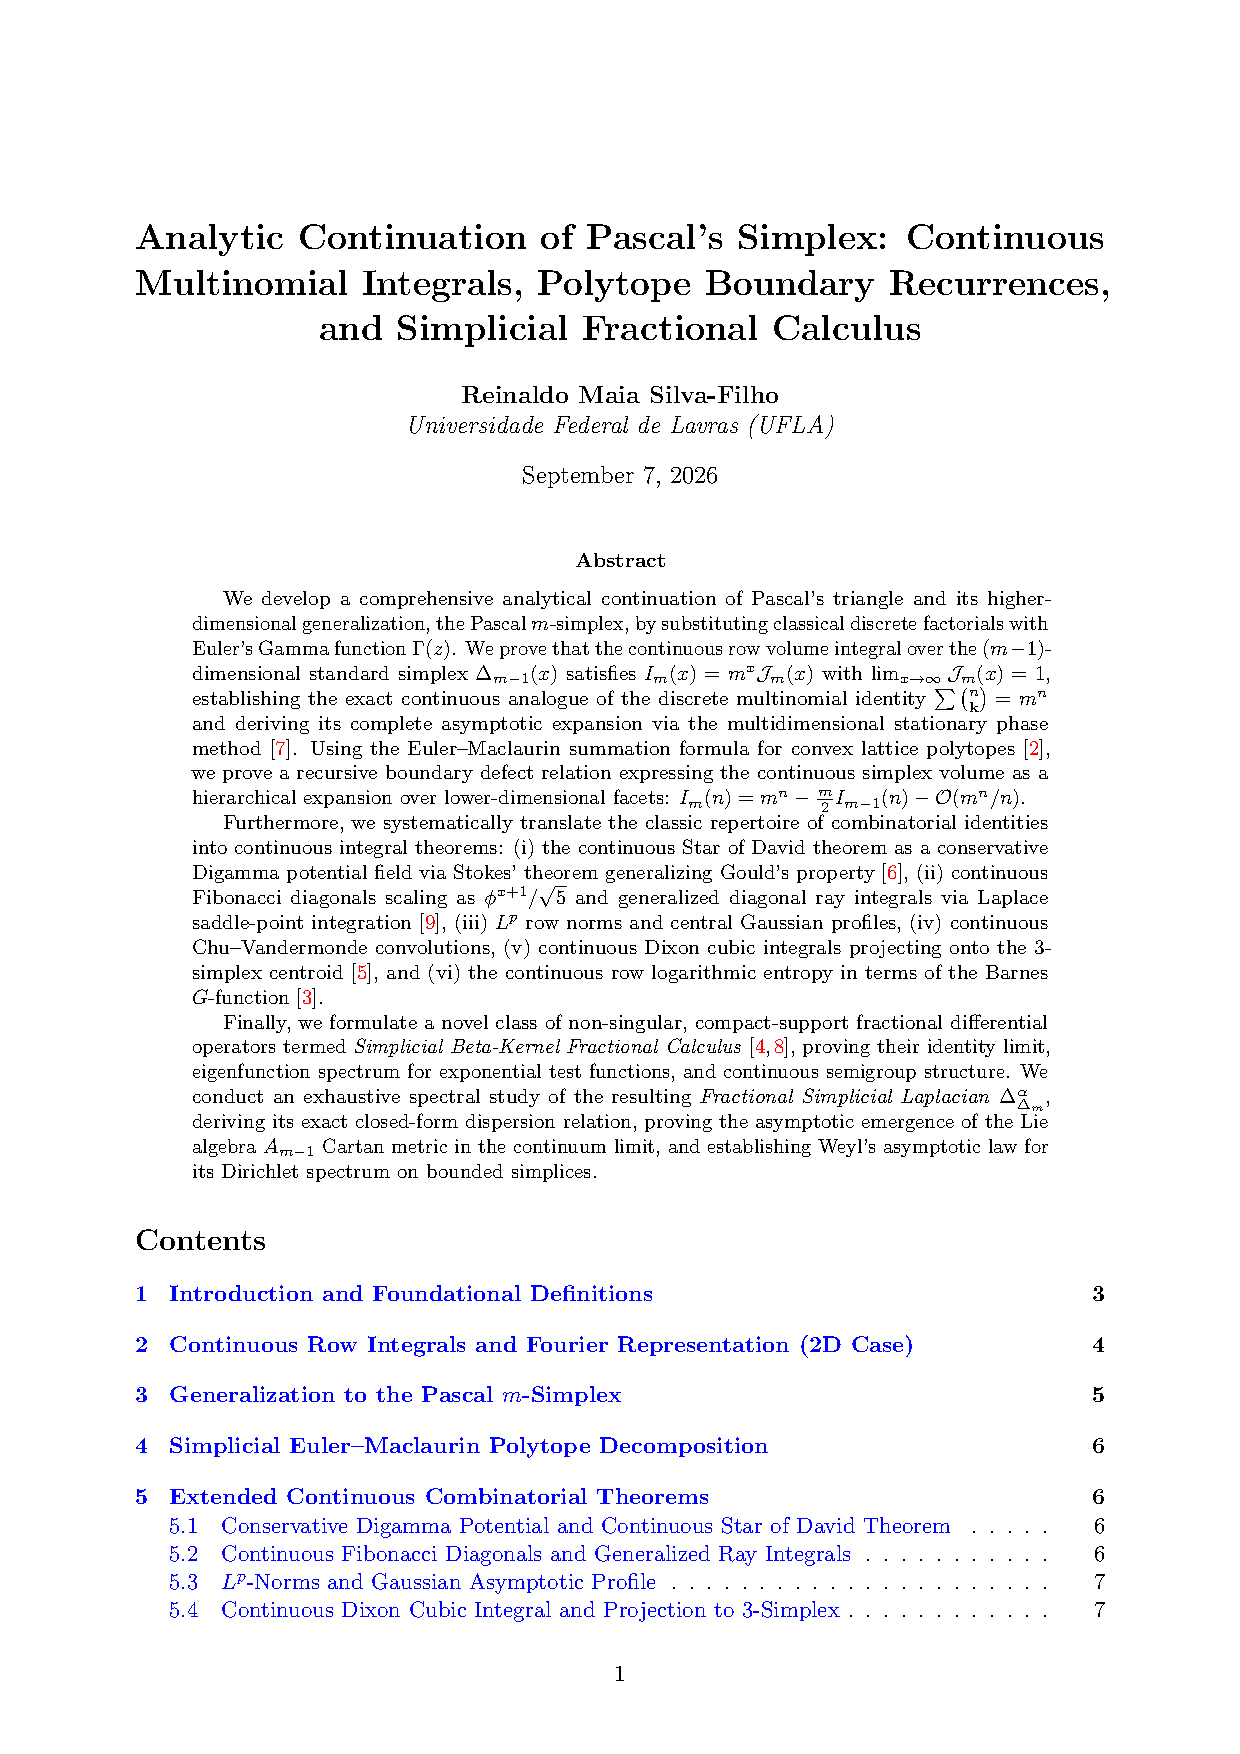
\includepdf[pages=1-]{chap03_pascal_simplex_continuous_multinomials.pdf}

\chapter[Fractional Waves and Porous Medium Transport]{Fractional Waves and Porous Medium Transport in Simplicial Environments}
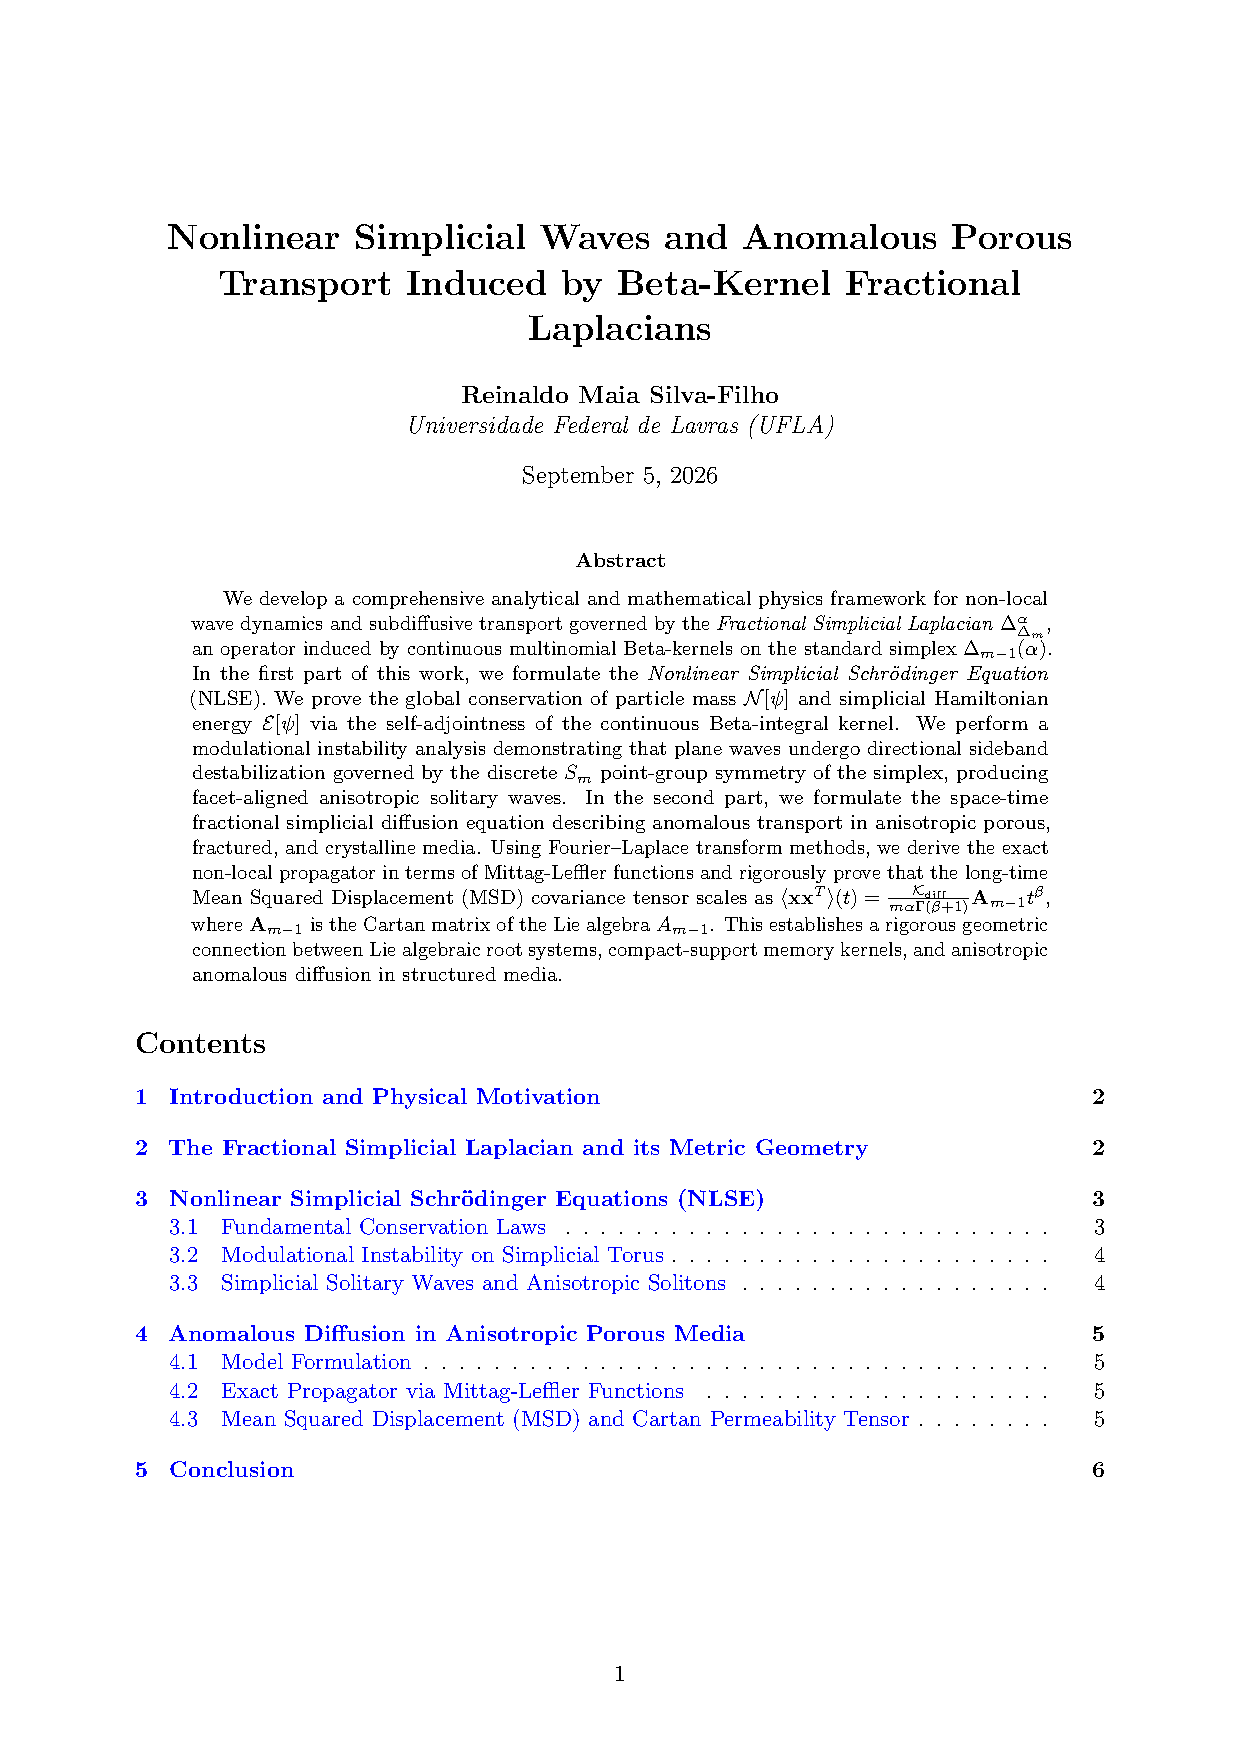
\includepdf[pages=1-]{chap04_simplicial_waves_porous_transport.pdf}

\chapter[Interdimensional Transforms and Lie Algebras]{Interdimensional Transforms, Barnes G-Function, and $A_{m-1}$ Lie Algebra}
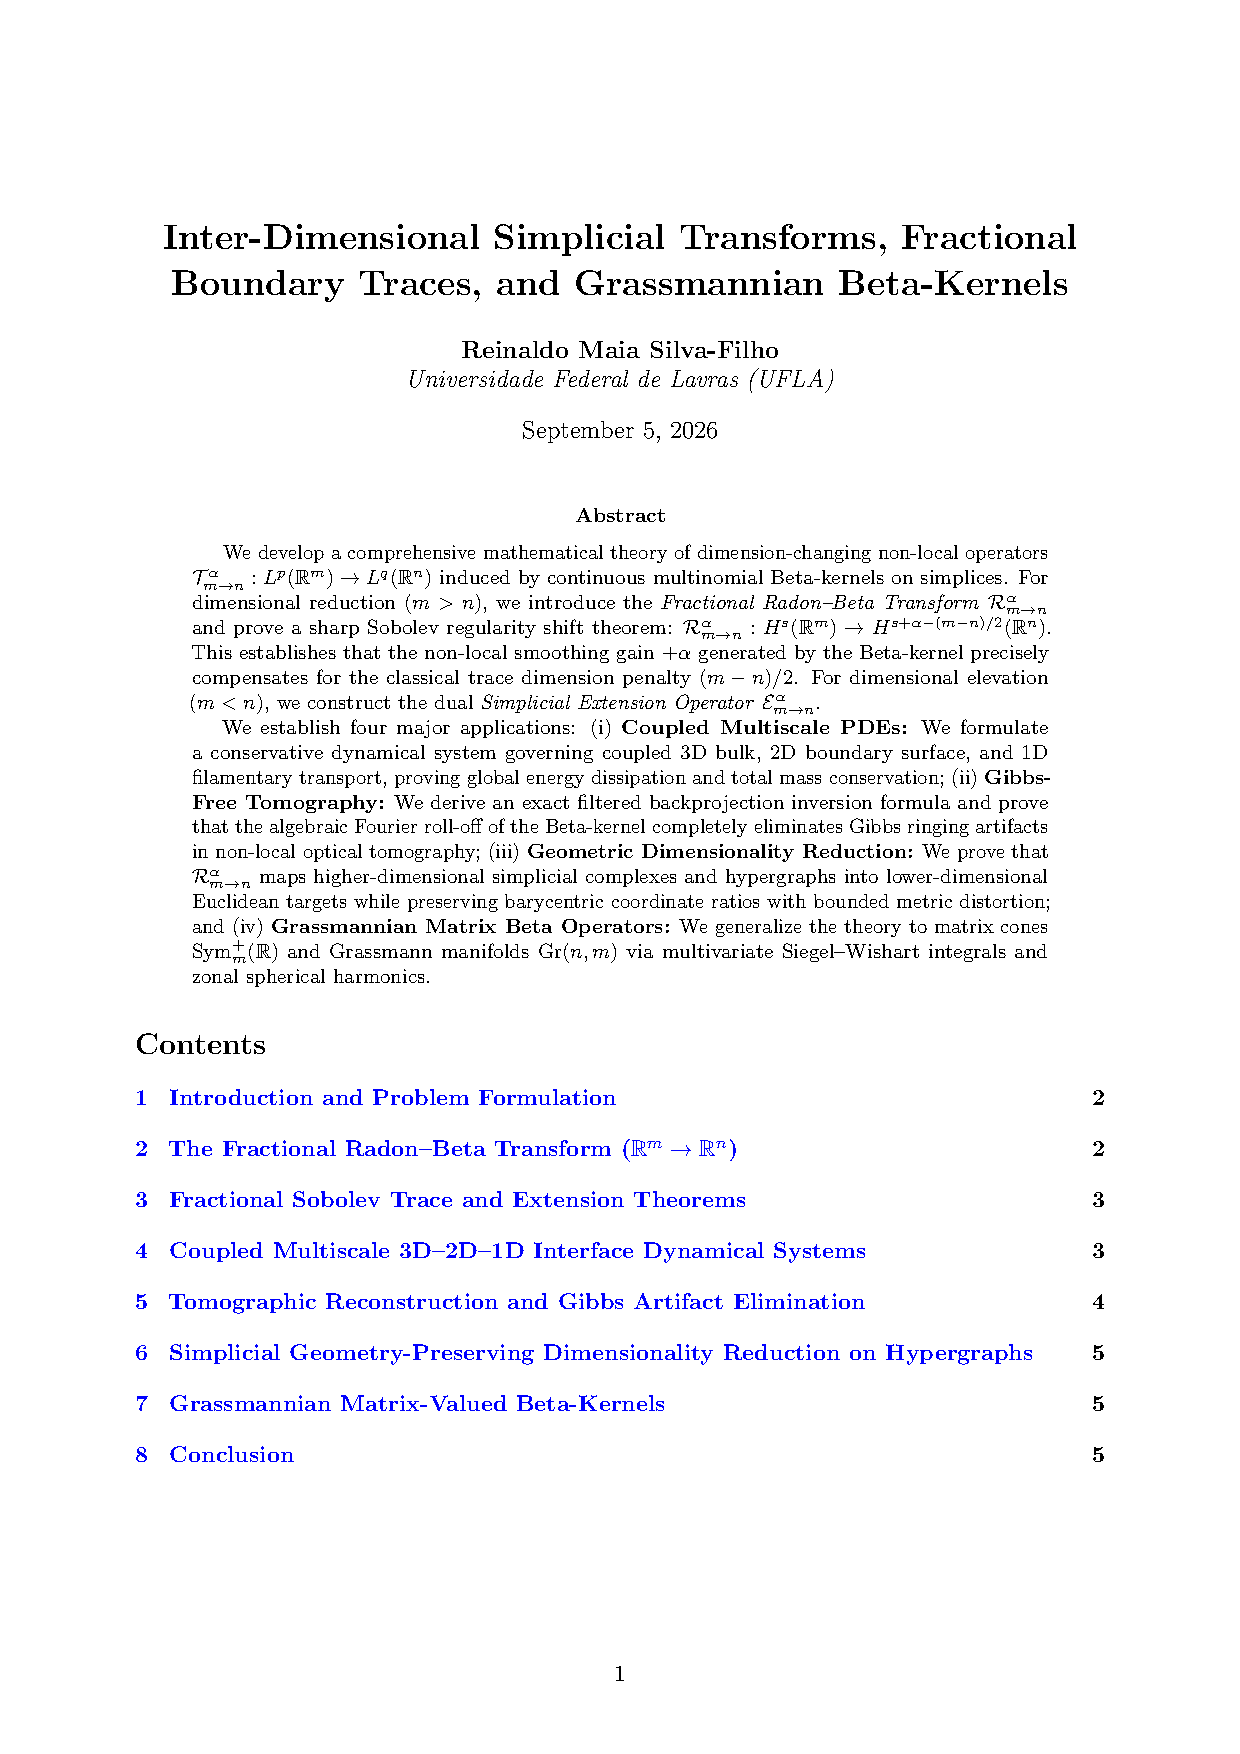
\includepdf[pages=1-]{chap05_interdimensional_transforms_barnes_lie.pdf}

\chapter[Spectral Geometry on the Sierpinski Simplex]{Spectral Geometry on the Sierpi\'nski Simplex and Dimensional Reduction}
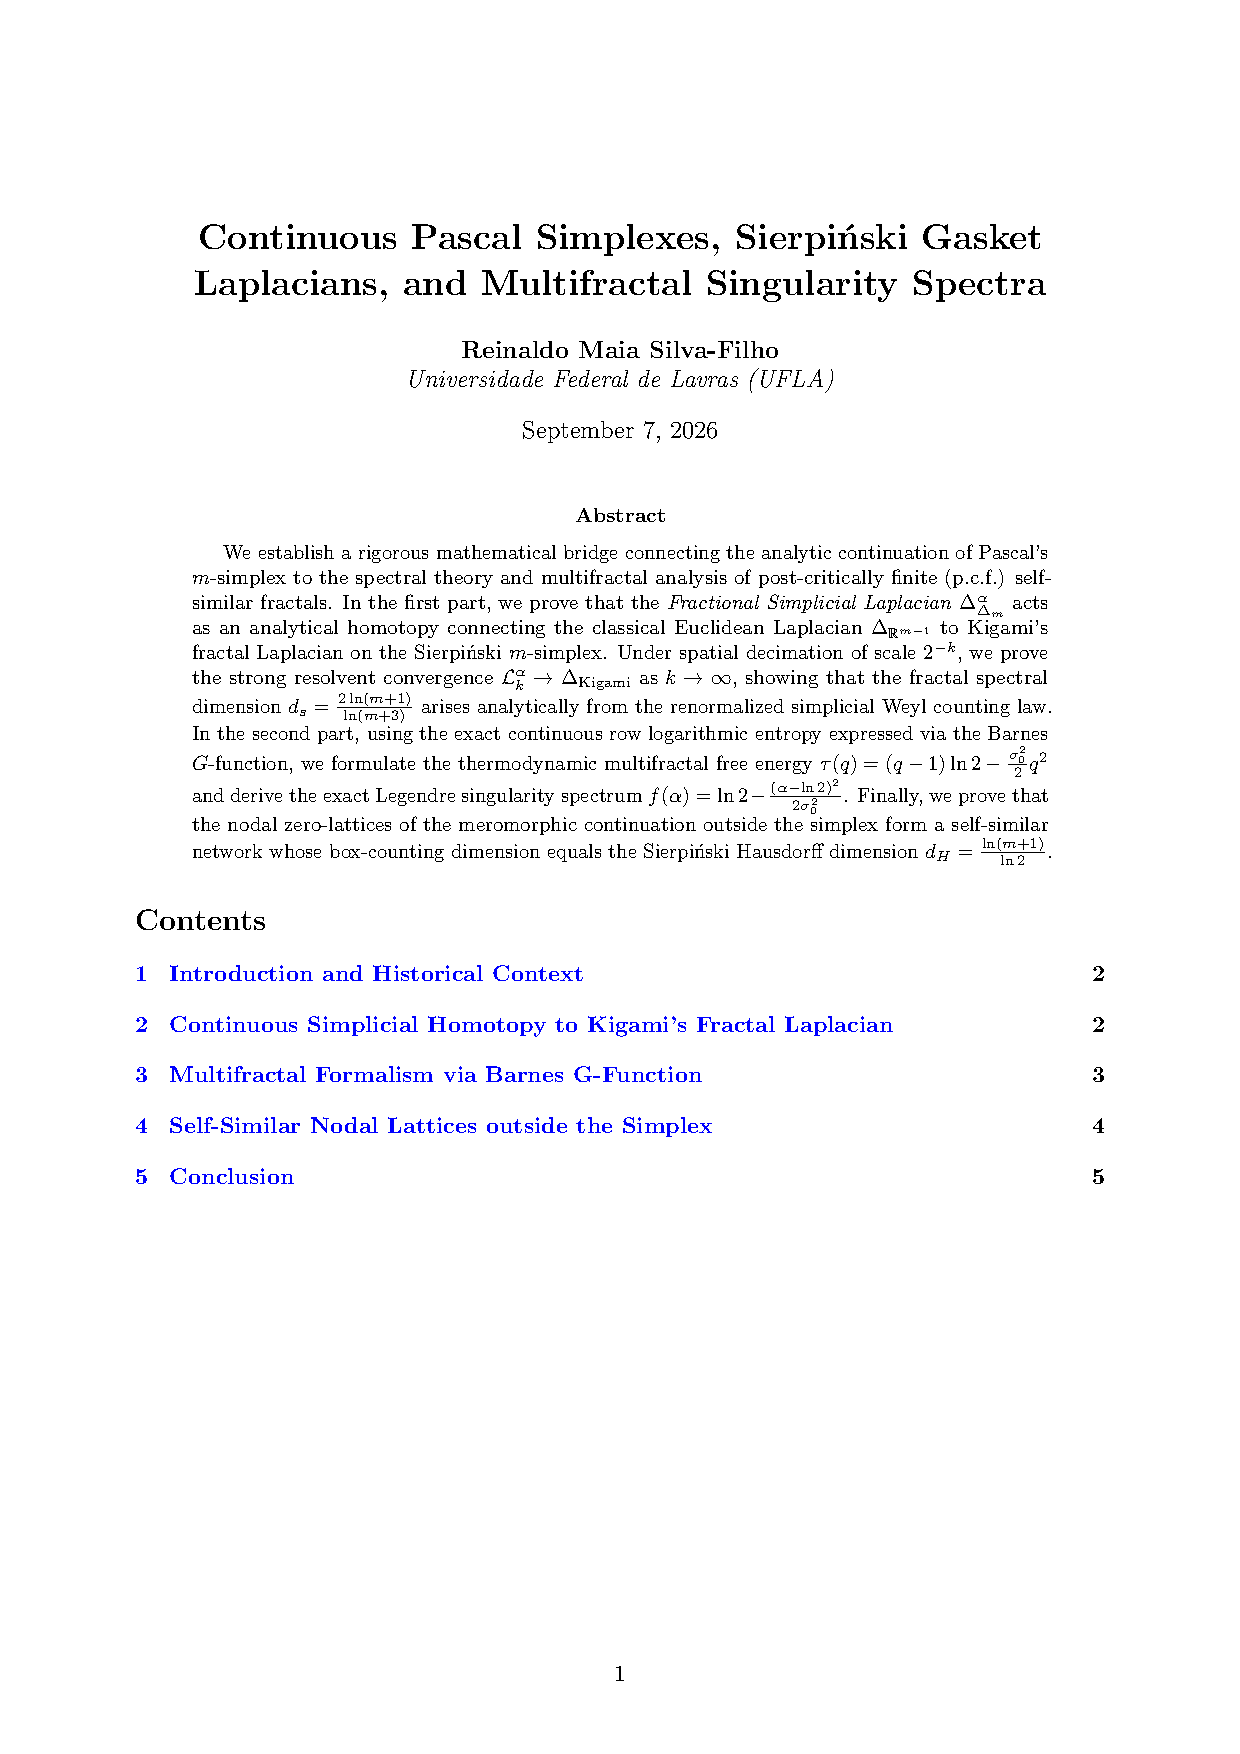
\includepdf[pages=1-]{chap06_sierpinski_fractal_resolvents_spectral_reduction.pdf}

% ==============================================================================
\part{Non-Euclidean Minimax Extrinsic Curvature and Relativistic Foliations}
% ==============================================================================

\chapter[Minimax-Flat Submanifolds in Obstacle Environments]{Minimax-Flat Submanifolds in Obstacle Environments and C1,1 Regularity}
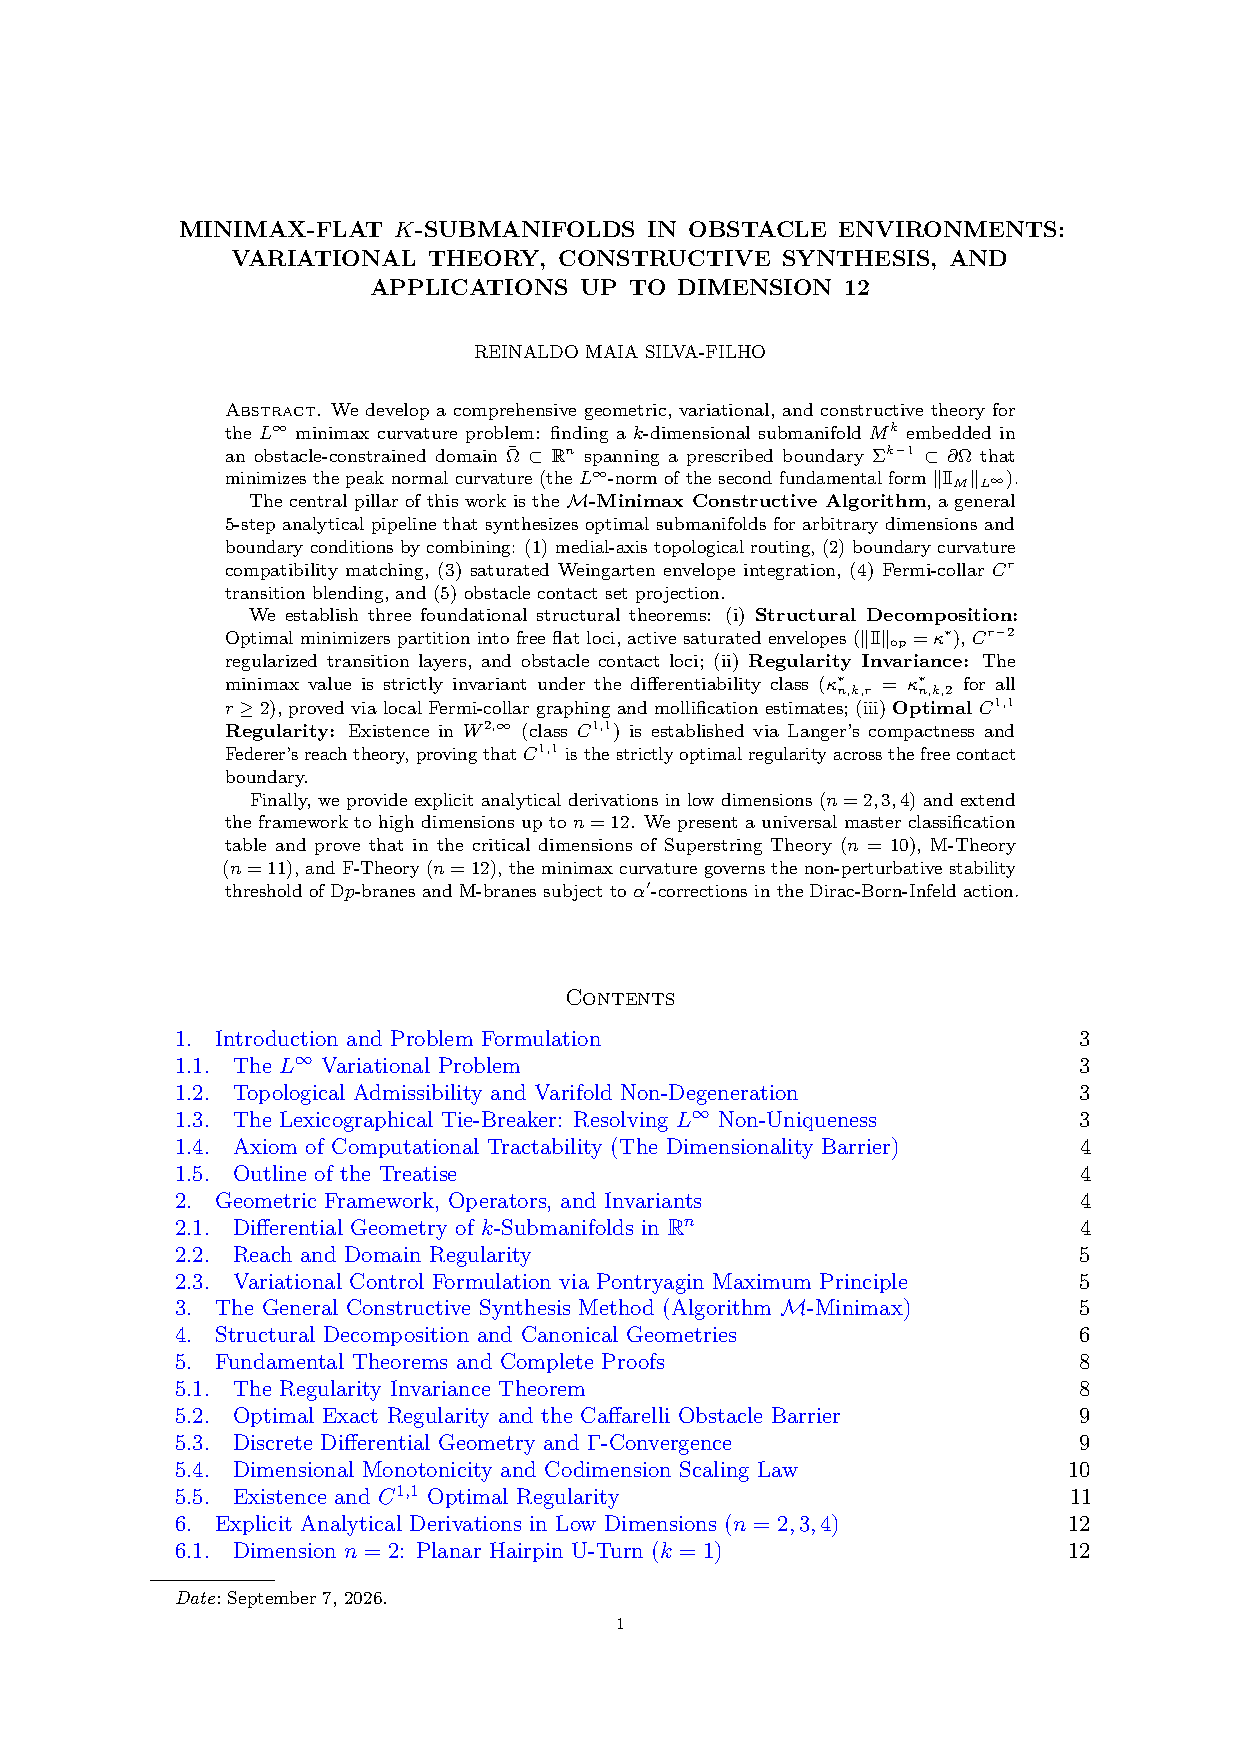
\includepdf[pages=1-]{chap07_minimax_extrinsic_curvature_submanifolds.pdf}

\chapter[Minimax Curvature and ADM Foliations]{Minimax Curvature in Non-Euclidean Geometries and ADM Spatial Foliations}
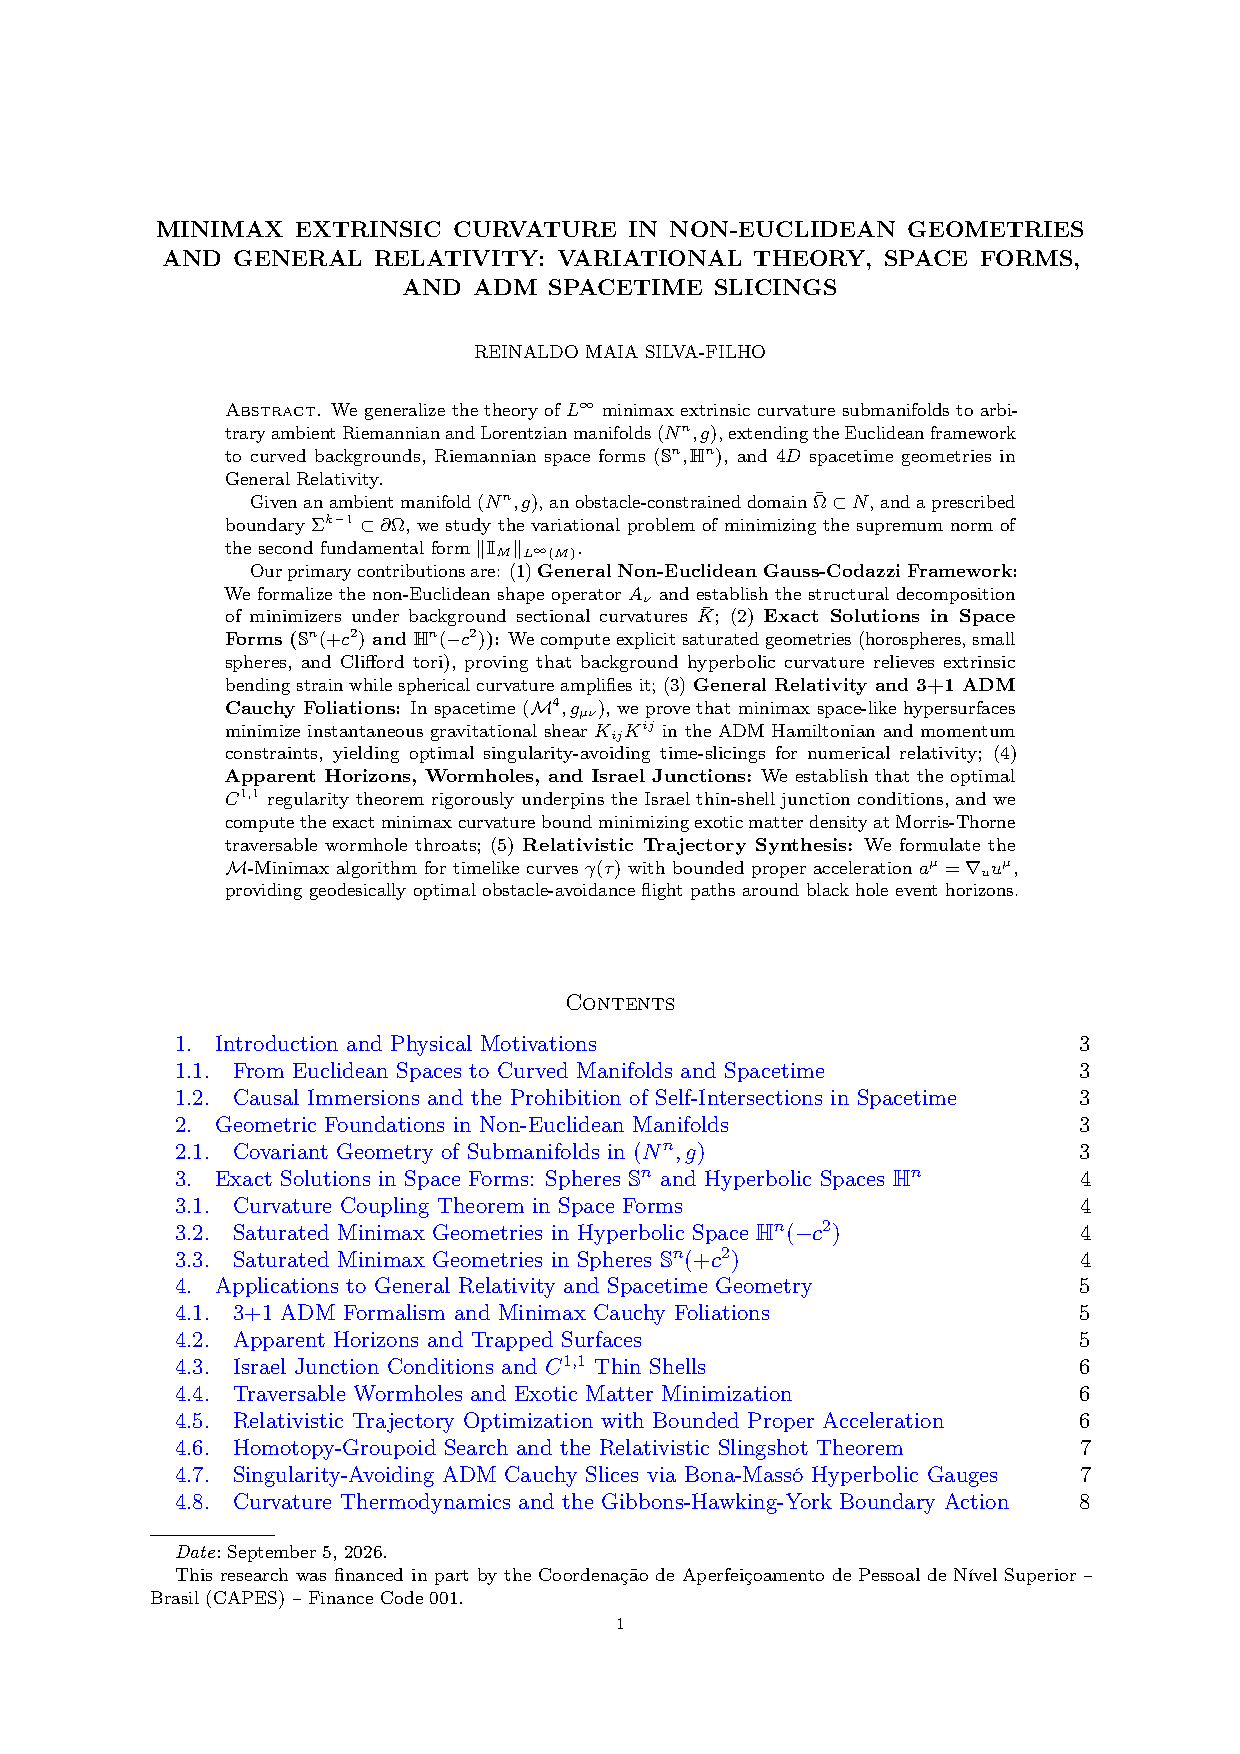
\includepdf[pages=1-]{chap08_noneuclidean_minimax_relativity_adm.pdf}

\chapter[Global Minimax Curvature and Jordan Loops]{Global Minimax Curvature, Covering Spaces, and Jordan Loops}
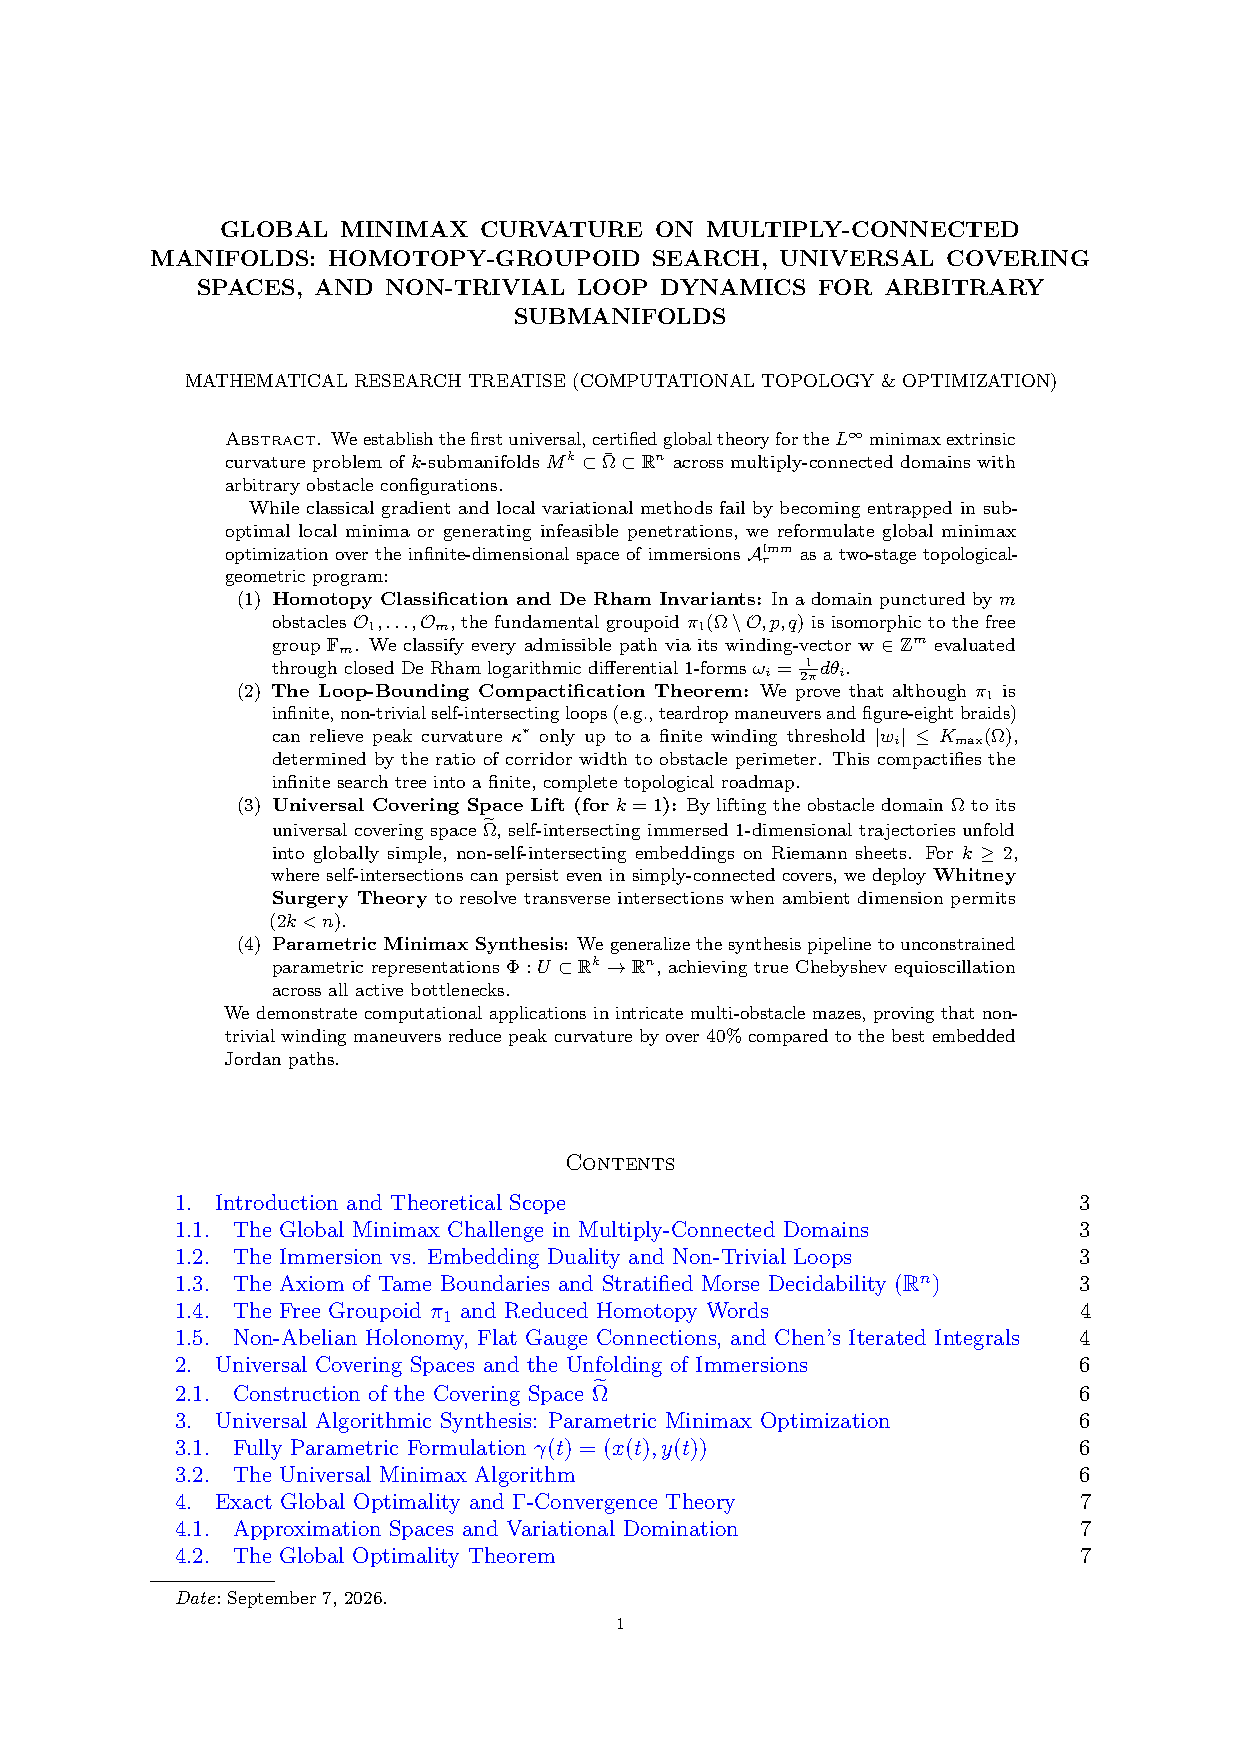
\includepdf[pages=1-]{chap09_global_homotopy_covering_spaces_jordan_loops.pdf}

\chapter[Minimax Trajectories in Information Geometry]{Minimax Trajectories in Information Geometry and Deep Learning}
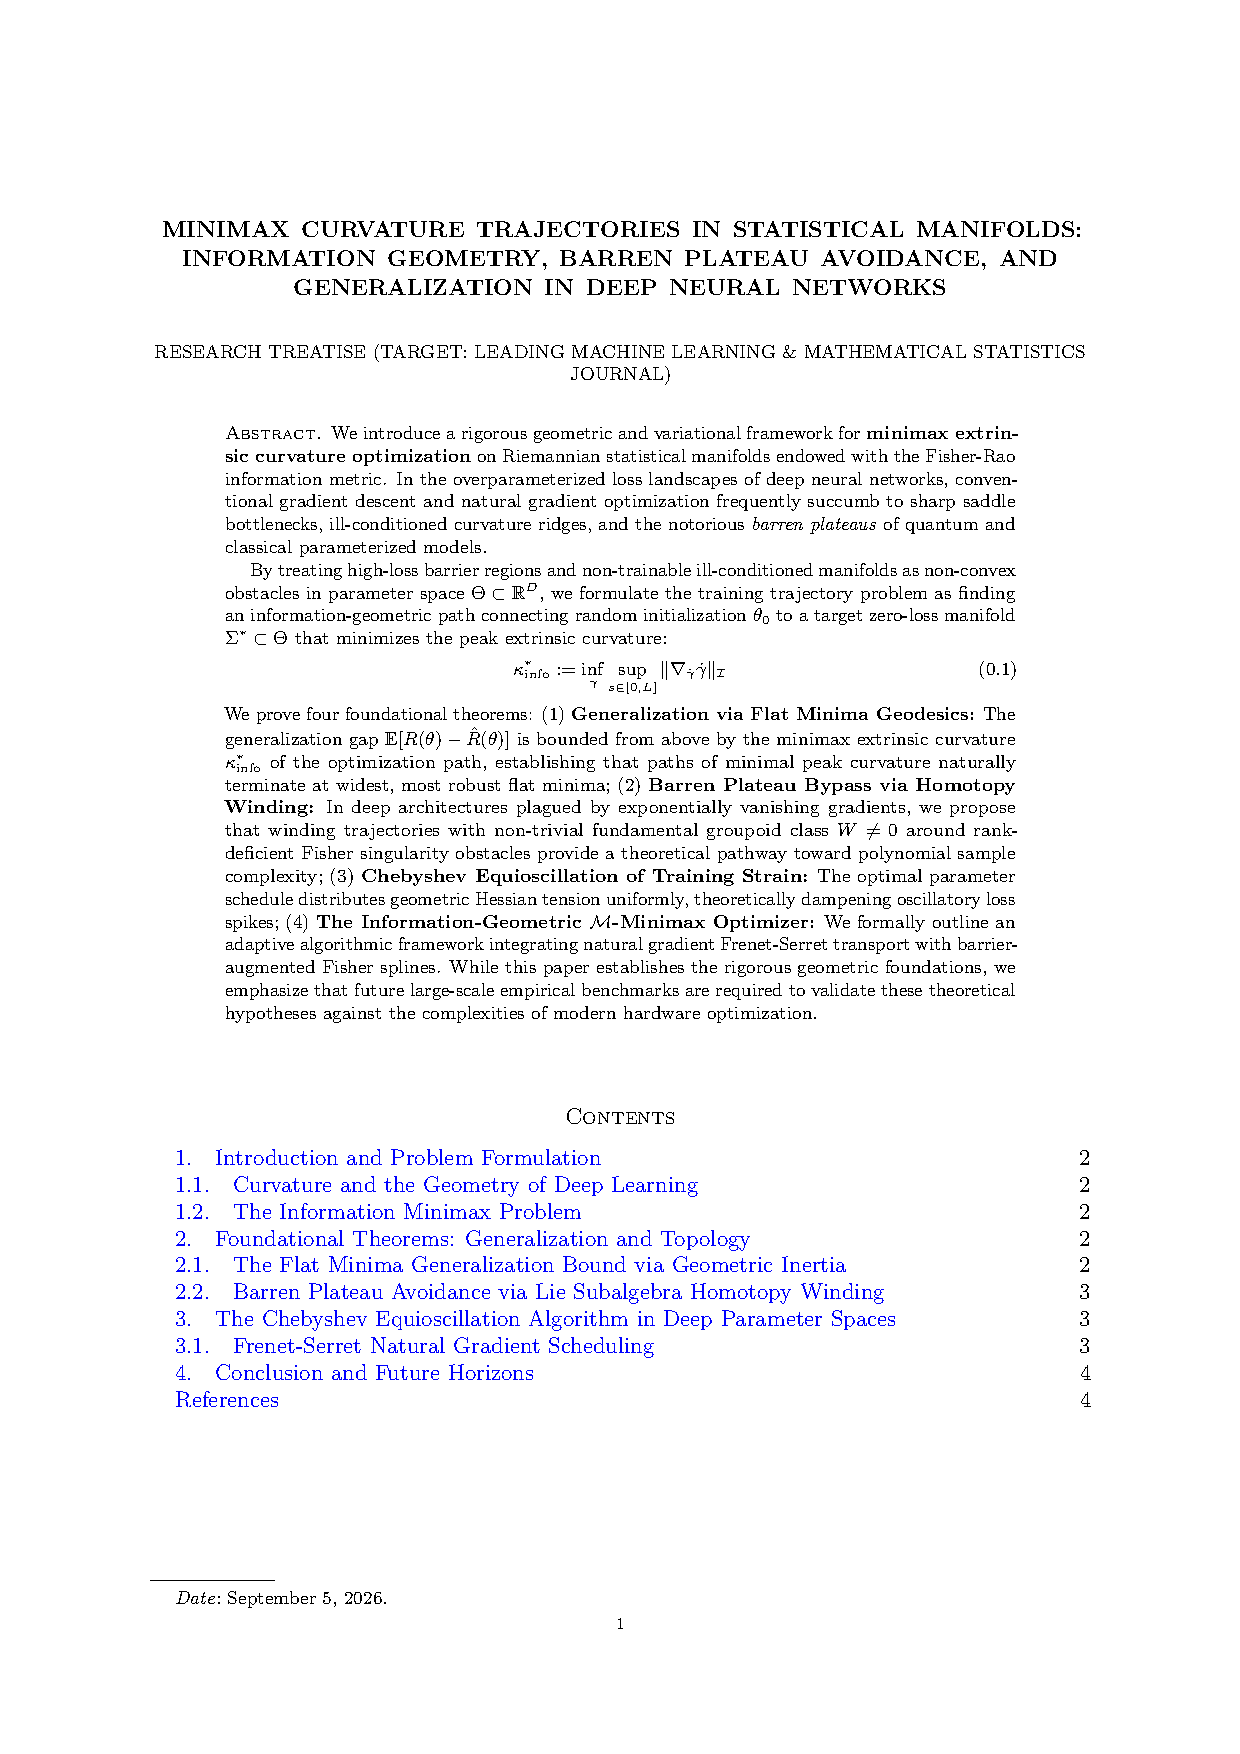
\includepdf[pages=1-]{chap10_information_geometry_minimax_deep_learning.pdf}

% ==============================================================================
\part{Emergent Spacetime, Holography, and the Grand Synthesis of Quantum Gravity}
% ==============================================================================

\chapter[Emergent Spacetime and Tensor Networks]{Emergent Spacetime and the Thermodynamics of Quantum Entanglement}
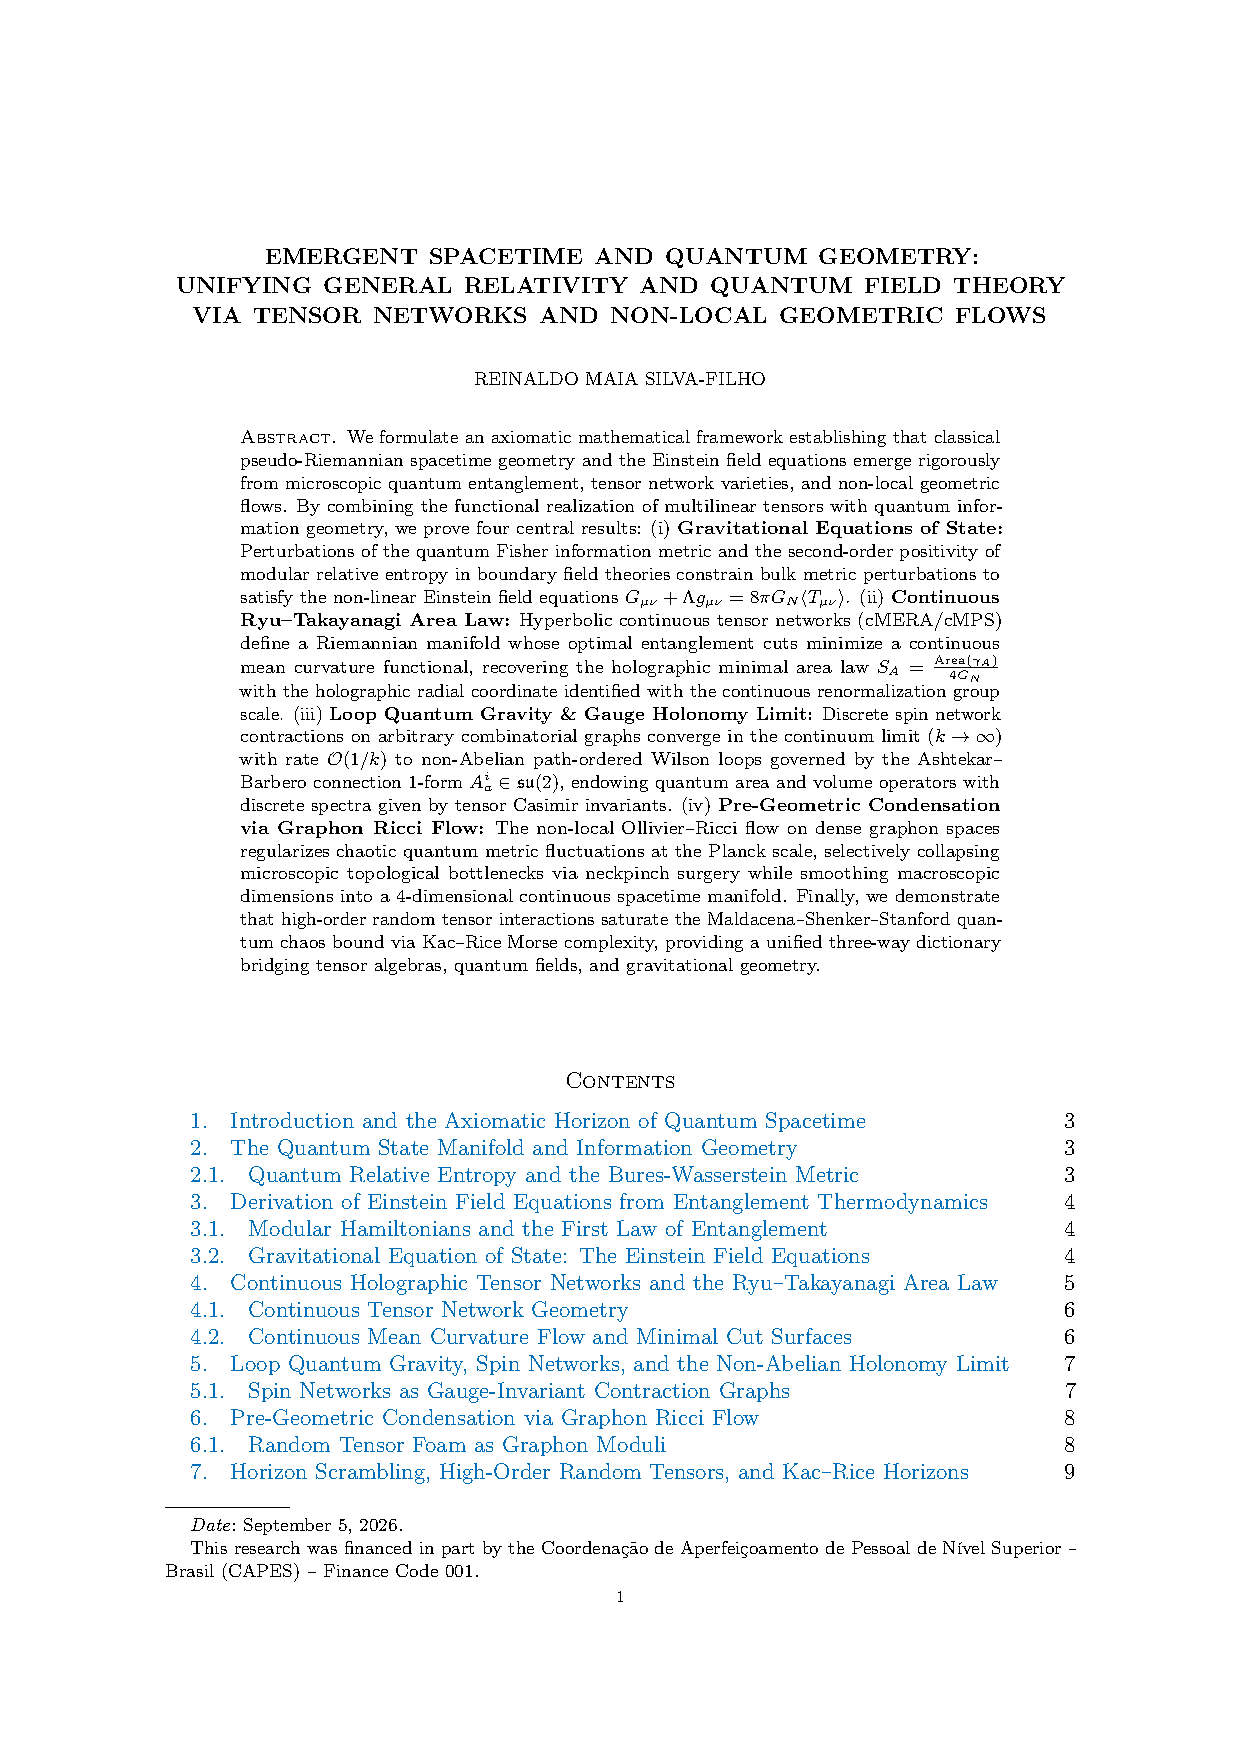
\includepdf[pages=1-]{chap11_emergent_spacetime_tensor_networks_holonomies.pdf}

\chapter[Grand Unification Treatise on Quantum Gravity]{Grand Unification Treatise on Quantum Gravity and Exact Analytical Solutions}
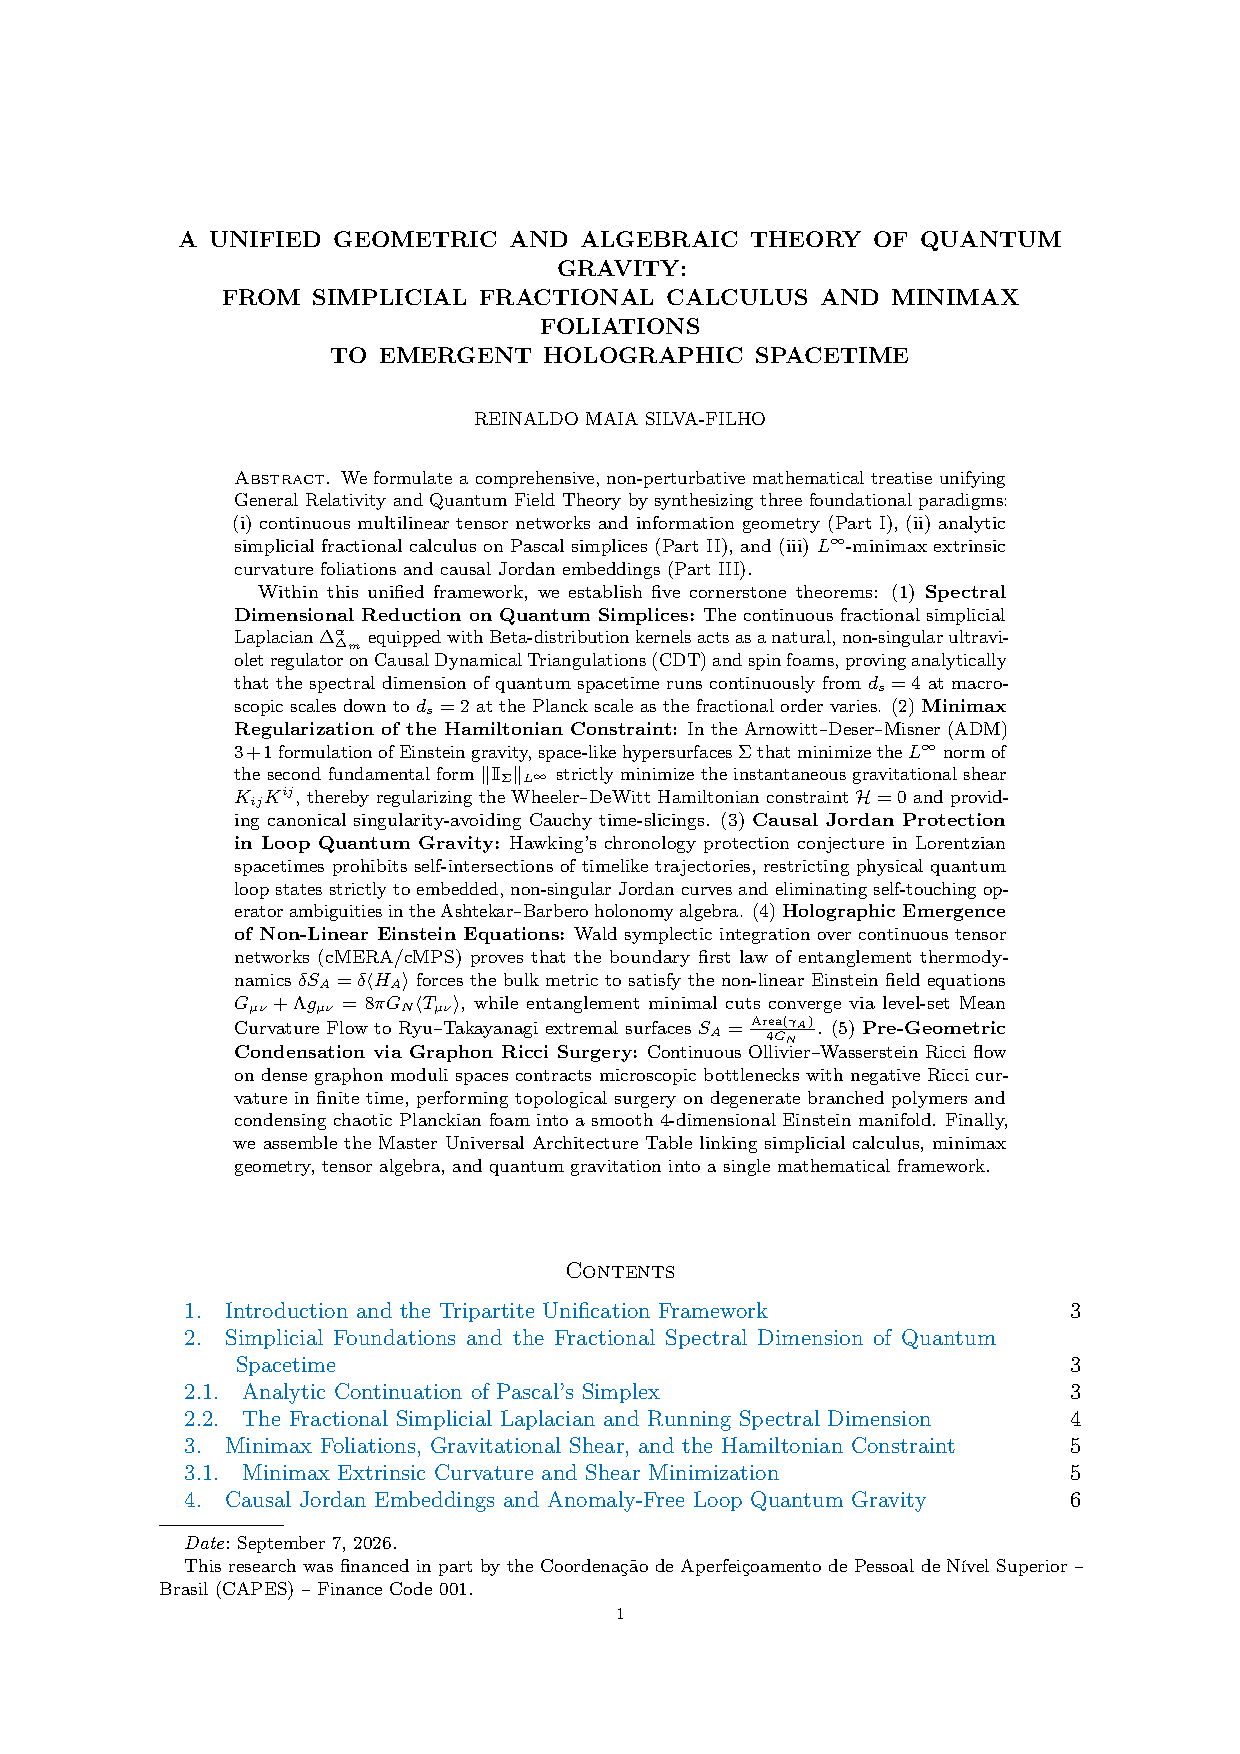
\includepdf[pages=1-]{chap12_grand_unification_quantum_gravity_treatise.pdf}

% ==============================================================================
\part{Observational Signatures and Experimental Testing Protocols}
% ==============================================================================

\chapter[Observational Signatures and Laboratory Tests]{Observational Signatures and Laboratory Tests of Unified Quantum Gravity}
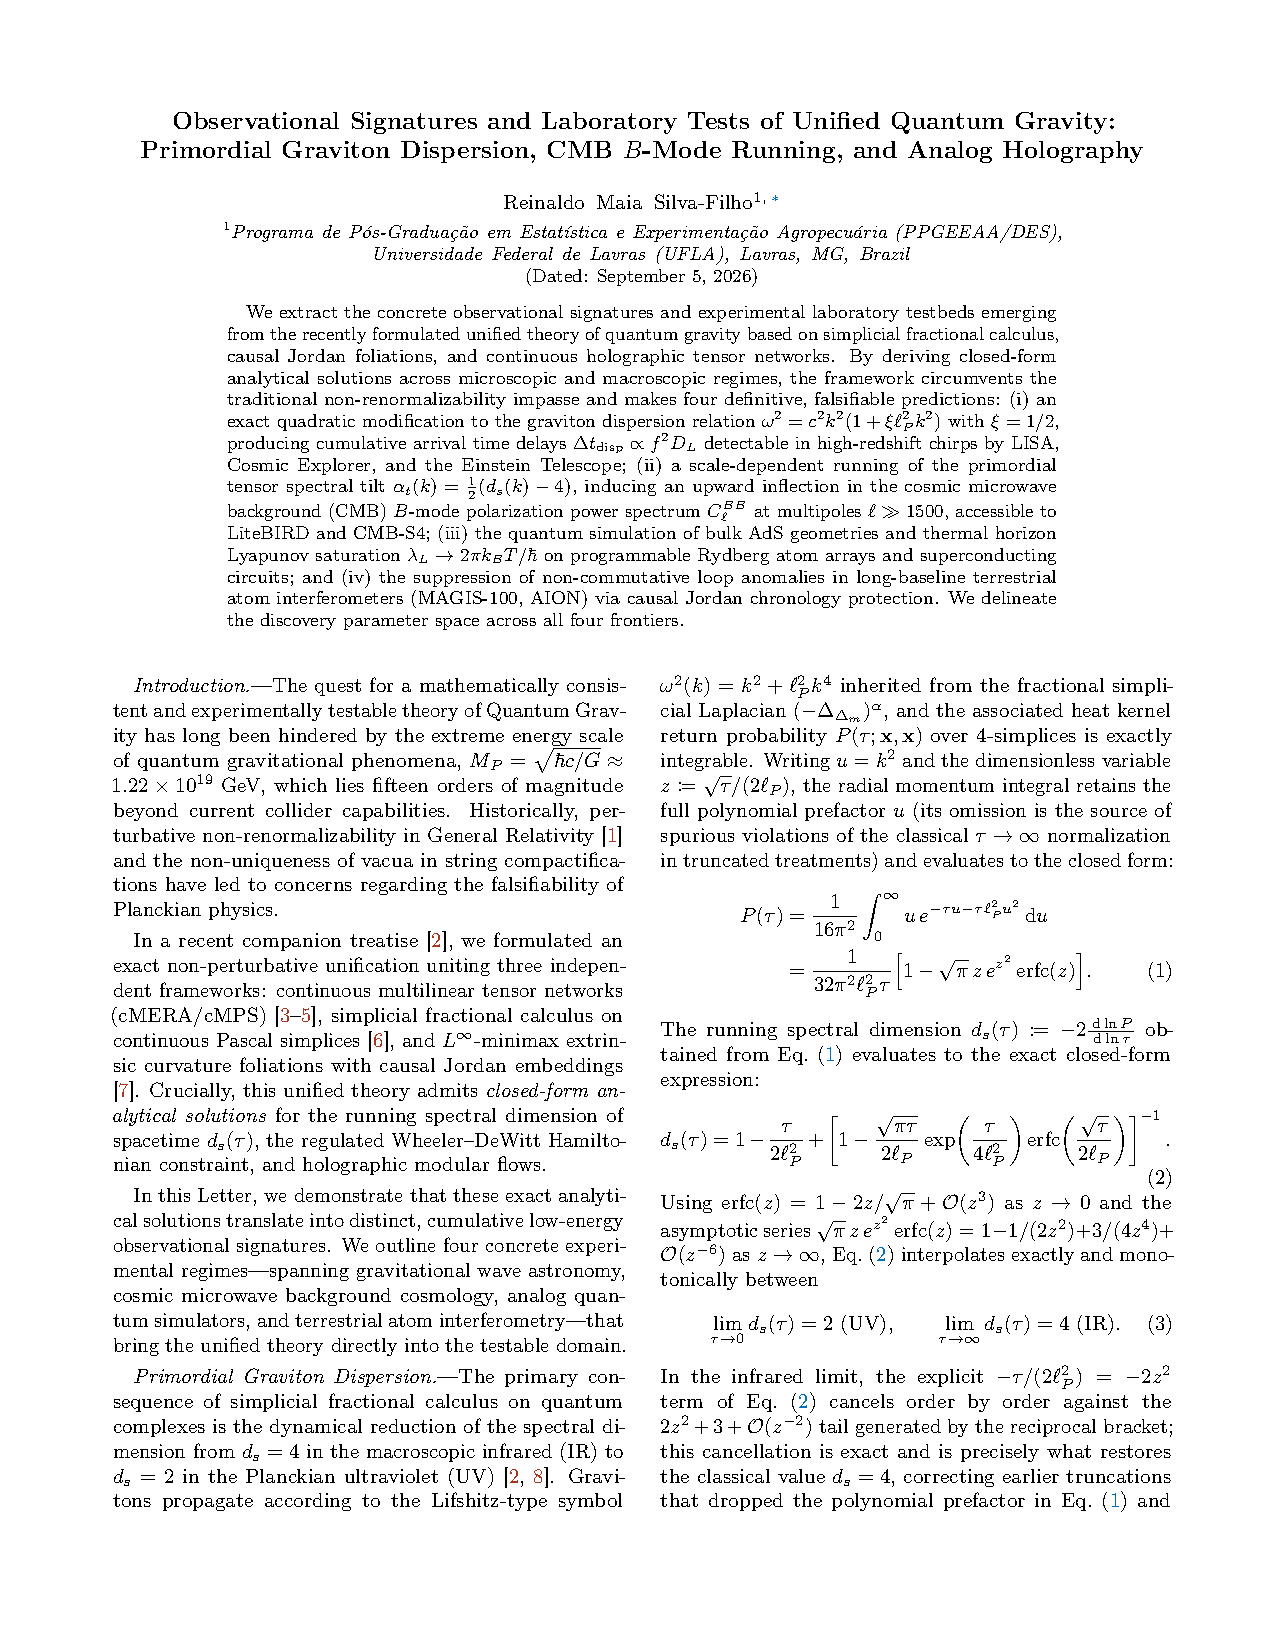
\includepdf[pages=1-]{chap13_experimental_observational_signatures_quantum_gravity.pdf}

\backmatter

\end{document}

